% debut d'un fichier latex standard
\documentclass[a4paper,12pt,twoside]{article}

% Pour les unités SI
\usepackage{siunitx}
% pour l'inclusion de figures en eps,pdf,jpg
\usepackage{graphicx}
% quelques symboles mathematiques en plus
\usepackage{amsmath}
% le tout en langue francaise
%\usepackage[english]{babel}
% on peut ecrire directement les caracteres avec l'accent
% a utiliser sur Linux/Windows
\usepackage[utf8]{inputenc}
\usepackage[T1]{fontenc}

% pour faire des systèmes d'équations
\usepackage{systeme}
\setcounter{tocdepth}{3} % Augmente le niveau affiché dans la table des matières

% a utiliser sur le Mac
%\usepackage[applemac]{inputenc}
% pour l'inclusion de links dans le document
\usepackage[colorlinks,bookmarks=false,linkcolor=blue,urlcolor=blue]{hyperref}
\usepackage{subcaption}
\paperheight=297mm
\paperwidth=210mm

\setlength{\textheight}{235mm}
\setlength{\topmargin}{-1.2cm} % pour centrer la page verticalement
%\setlength{\footskip}{5mm}
\setlength{\textwidth}{15cm}
\setlength{\oddsidemargin}{0.56cm}
\setlength{\evensidemargin}{0.56cm}

\pagestyle{plain}

% quelques abreviations utiles
\def \be {\begin{equation}}
\def \ee {\end{equation}}
\def \dd  {{\rm d}}

\newcommand{\mail}[1]{{\href{mailto:#1}{#1}}}
\newcommand{\ftplink}[1]{{\href{ftp://#1}{#1}}}
%
% latex SqueletteRapport.tex      % compile la source LaTeX
% xdvi SqueletteRapport.dvi &     % visualise le resultat
% dvips -t a4 -o SqueletteRapport.ps SqueletteRapport % produit un PostScript
% ps2pdf SqueletteRapport.ps      % convertit en pdf

% pdflatex SqueletteRapport.pdf    % compile et produit un pdf


% ======= Le document commence ici ======

\begin{document}
% Le titre, l'auteur et la date
\title{Exercise 3: Pendulum with a vertical excitation\\{\small Physique Numérique I}}
\date{\today}
\author{Delphine Martres et Damien Korber\\{\small \mail{delphine.martres@epfl.ch} et \mail{damien.korber@epfl.ch}}}
\maketitle
\tableofcontents % Table des matieres
\newpage % Si la toc est trop grande, voir ligne 19.
% Quelques options pour les espacements entre lignes, l'identation
% des nouveaux paragraphes, et l'espacement entre paragraphes
\baselineskip=16pt
\parindent=15pt
\parskip=5pt



%%%% ON COMMENCE A ECRIRE D'ICI

\section{Introduction}

\section{Analytical computations}

\section{Numerical computations}

\subsection{Little movements without excitation or air resistance}
In this section, no excitation or air resistance will be considered: $\kappa = 0$, $d = 0$.
The movements are small, and approximations are made: $\theta_0 = \num{d-6}$, $\dot{\theta}_0 = 0$.
The computations run for \SI{20}{\second}.

\subsubsection{Comparison between the analytical solution and the approximation of Stormer-Verlet method}
\begin{figure}[h]
\begin{subfigure}[t]{0.48\textwidth}
	\includegraphics[width=\textwidth]{graphs/a_traj_full.eps}
	\caption{Angle of the pendulum with respect to time, with a comparison between the Stormer-Verlet numerical method and the analytical solution.}
	\label{fig:a-traj-full}
\end{subfigure}
~
\begin{subfigure}[t]{0.48\textwidth}
	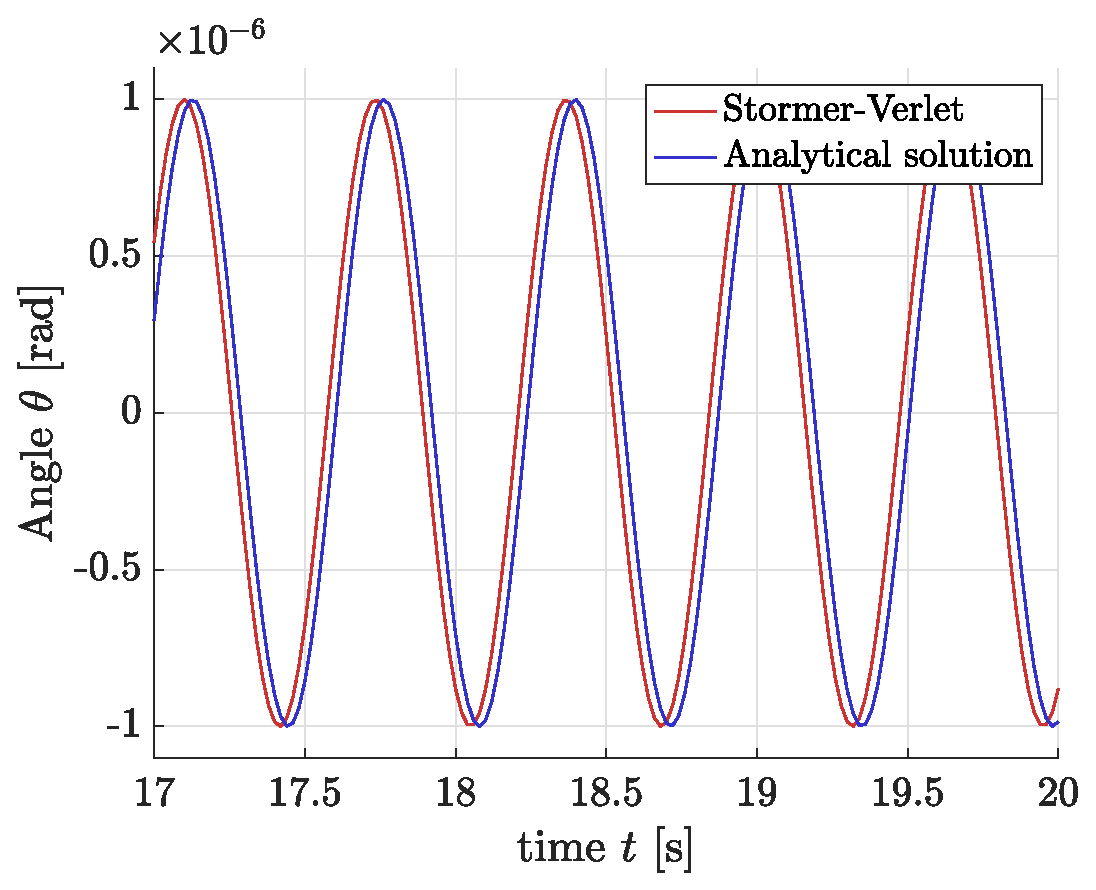
\includegraphics[width=\textwidth]{graphs/a_traj_zoomed.eps}
	\caption{Same plot as \ref{fig:a-traj-full}, with the beginning cropped out to get a better view of the small difference between the numerical and analytical solutions.}
	\label{fig:a-traj-zoomed}
\end{subfigure}
\caption{Angle of the pendulum with respect to time.}
\label{fig:a-traj}
\end{figure}

\subsubsection{Convergence study}

\subsubsection{Conservation of energy}

\subsection{Great movements}

\subsection{Resonant excitation}

\subsection{Parametric excitation}

\subsection{Poincaré section: chaos without air resistance}

\subsection{Pointcaré section: chaos with air resistance}

\end{document}
